\chapter{Universal Module}\label{chap:universal_module}

The chapter \ref{chap:rofi} gives the specification for modules in the RoFI
platform. In this chapter, we present the RoFI \emph{universal module}. This
module is supposed to be the main building block of RoFI systems. It should
provide enough versatility to build vast amount of systems.

This chapter provides overview of the design of the universal module and gives a
specification to implement it. The current state of implementation is discussed
in the chapter \ref{chap:prototypes}.

\section{Universal Module Shape}

The universal RoFI module occupies two adjacent cells of the grid as can be seen
in the figure \ref{fig:um_reference}. Please note that this drawing gives a
simplified model in which many technical details are omitted. The arrangement of
the module is inspired by the M-TRANs \cite{kurokawa_distributed_2008}. Unlike
M-TRANs, the universal module is grid-aware. There are four parts from which the
module is composed:
\begin{enumerate*}
    \item \emph{body A},
    \item \emph{body B},
    \item \emph{shoe A} and
    \item \emph{shoe B}.
\end{enumerate*}
See figure \ref{fig:um_body_parts}. Bodies are supposed to encapsulate
actuators, electronics and accumulators; shoes are meant to provide connection
to other modules and provide movement.

\begin{figure}
    \centering
    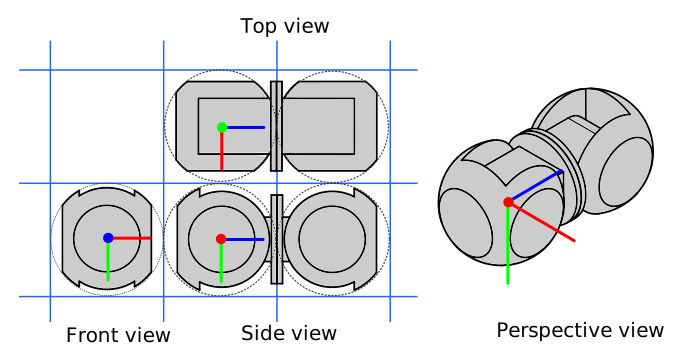
\includegraphics[width=\textwidth]{figures/um_reference.pdf}
    \caption{The universal RoFI module. Blue lines specify the grid, dotted
    lines marks spheres in which the module in inscribed. Note that we show the
    module with the Z axe facing right as it better fits  the page layout. }
    \label{fig:um_reference}
\end{figure}

\begin{figure}
    \centering
    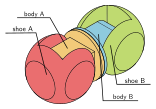
\includegraphics[width=0.7\textwidth]{figures/um_body_parts.pdf}
    \caption{Parts of the universal module.}
    \label{fig:um_body_parts}
\end{figure}

There are 3 degrees of freedom (figure \ref{fig:um_axis}):
\begin{enumerate}
    \item shoe A can rotate against body A along the $\alpha$ axe in a range
    $\langle -90^\circ; +90^\circ\rangle$,
    \item shoe B can rorate against body B along the $\beta$ axe in a range
    $\langle -90^\circ; +90^\circ\rangle$ and
    \item body A can rotate against body B along the $\gamma$ axe in $\langle
    -180^\circ; +180^\circ\rangle$ with an overflow\footnote{First prototypes
    feature a limitation on a number of overflows in one direction the $\gamma$
    axe due to technical limitations. }.
\end{enumerate}
The module should be able to provide at least 1.5 $\text{N}\cdot\text{m}$ of
torque for each axe.

\begin{figure}
    \centering
    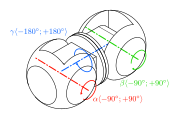
\includegraphics[width=0.7\textwidth]{figures/um_axis.pdf}
    \caption{Degrees of freedom of the universal module. The figure represents neutral position of each joint.}
    \label{fig:um_axis}
\end{figure}

There are 3 docks on each each shoe -- docks $X+, X-$ and $Z-$. The position of
the docks is captured in the figure \ref{fig:um_docks}. Given this setup we
can construct universal module descriptor shown in the figure
\ref{fig:um_descriptor}.

\begin{figure}
    \centering
    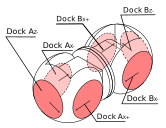
\includegraphics[width=0.7\textwidth]{figures/um_docks.pdf}
    \caption{Docks on the universal module. The arrow on each dock specifies its orientation.}
    \label{fig:um_docks}
\end{figure}

\section{Intramodule Architecture}

\section{The RoFI "BIOS" \todo{Proper naming}}

\section{RoFI lib}

\todo{Something here}